% ----------------------------------------------------------------------------------------------------------------
% This .tex file (and associated .cls V3.2SP) *DOES NOT* produce:
%       1) The Permission Statement
%       2) The Conference (location) Info information
%       3) The Copyright Line with ACM data
%       4) Page numbering
% ---------------------------------------------------------------------------------------------------------------

%\documentclass{acm_proc_article-sp}
\documentclass{sig-alternate}

\usepackage{url}
\usepackage{graphicx}
\usepackage{amssymb}
\usepackage{stackrel}
\usepackage{array}
\usepackage{amsmath}
\usepackage{verbatim}
\usepackage{multirow}
\usepackage{fancybox}
\usepackage{algorithmic}
\usepackage{algorithm}
\usepackage{blkarray}
%\usepackage{pdflscape}
%\usepackage{amsthm}
%\usepackage{fullpage}
%\usepackage{rotating}

\begin{document}

%\title{Mining Semantically Associated Itemsets from Ontology-Annotated Data}
\title{Mining Biomedical Ontologies and Data with Unified RDF Hypergraphs}

\numberofauthors{5}
\author{
% one 'row of three' or two rows (consisting of one row of three and a second row of one, two or three).
% 1st. author
\alignauthor
Haishan Liu\\
       \affaddr{University of Oregon}\\
       \affaddr{Eugene, OR, 97403, USA}\\
       \email{ahoyleo@cs.uoregon.edu}
% 2nd. author
\alignauthor Dejing Dou\\
       \affaddr{University of Oregon}\\
       \affaddr{Eugene, OR, 97403, USA}\\
       \email{dou@cs.uoregon.edu}
% 3rd. author
\alignauthor Ruoming Jin\\
       \affaddr{Kent State University}\\
       \affaddr{Kent, OH, 44242, USA}\\
       \email{jin@cs.kent.edu}
\and  % use '\and' if you need 'another row' of author names
% 4th. author
\alignauthor Paea LePendu\\
       \affaddr{Stanford University}\\
       \affaddr{Stanford, CA, 94305, USA}\\
       \email{plependu@stanford.edu}
\alignauthor Nigam Shah\\
       \affaddr{Stanford University}\\
       \affaddr{Stanford, CA, 94305, USA}\\
       \email{nigam@stanford.edu}
}
\date{20 February 2013}

\maketitle
\begin{abstract}

Ontologies as formal specification of domain knowledge have been well used for annotating real-life data especially in the biomedical domain. As researchers analyze huge amounts of data that are annotated by large biomedical ontologies, one of the major challenges for data mining is to leverage both ontologies and data together in a systematic and scalable way. In this paper, we address two interesting and related problems for mining biomedical ontologies and data: i) how to discover \emph{semantic associations} with the help of formal ontologies; ii) how to identify potential errors in the ontologies with the help of data. By representing both ontologies and data in \textit{RDF hypergraphs} and subsequently transforming the hypergraphs to corresponding bipartite or tripartite forms for the purpose of designing pertinent mining algorithms,  we provide a generalized data mining method that scales beyond what existing ontology-based approaches can provide. We use random walk with restart to efficiently calculate the similarity between concepts so as to determine their associations from very large size of data and ontologies. We show the proposed method is indeed capable of capturing semantic (indirect) associations while seamlessly incorporate domain knowledge defined in ontologies through experiments performed with real life data and ontologies. We also show that our data mining methods can discover the errors in biomedical ontologies injected by human operations. This research also contributes to an emerging research direction of \emph{semantic data mining}, in which formal semantics that exist in data and knowledge can be represented and incorporated into the data mining process in a seamless way.


%In this paper, we address an interesting data mining problem of finding semantically associated itemsets (i.e., items connected via indirect links) on ontology-annotated datasets. Semantically rich datasets, such as those annotated by formal ontologies and represented in RDF or OWL, can be viewed as datasets embedded with domain knowledge. This new standard of representation provides a unique opportunity to mine the data and domain knowledge simultaneously. In this paper, we develop a way to represent both data and ontology in a unified graph representation, and we propose to use random walk with restart to efficiently calculate the similarity between items so as to determine their associations from very large size of data and ontologies.
%We show the proposed method is indeed capable of capturing semantically associated itemsets while seamlessly incorporate domain knowledge defined in ontologies through experiments performed with real life data and ontologies. The semantically associated itemsets discovered in our experiment is promising to provide valuable insights on interrelationship between medical concepts and other domain specific ones.

\end{abstract}

%\category{H.2.8}{Database Management}{Data Mining}
%\terms{Algorithms, Theory}

\keywords{Semantic Data Mining, RDF Hypergraphs, Semantic Associations, Biomedical Ontologies} % NOT required for Proceedings

%\theoremstyle{definition}
\newtheorem{myexp}{Example}[section]
\newtheorem{mydef}{Definition}[section]
\newtheorem{mythm}{Theorem}[section]
\newtheorem{mylem}{Lemma}[section]
\section{Introduction}
\label{sec:intro}

Researchers around the world are linking more and more data to ontologies which are formal specification of concepts and relationships in various domains. Formal ontologies have been extensively developed and harnessed in scientific research, particularly in biomedical research. Knowledge evolves rapidly in biomedicine and has promoted the creation and use of ontologies to advance scientific progress.  Besides the size of data increases exponentially, an increasing number of ``large" biomedical ontologies are developed. Prominent examples of this effort include the Gene Ontology (GO)~\cite{GO} and the Unified Medical Language System (UMLS)~\cite{UMLS}. Over 300 ontologies have been loaded into the National Center of Biomedical Ontology (NCBO) BioPortal library at Stanford~\cite{Noy2009}, specifying more than 5.6 million terms in the biomedical domain.

There are two major challenges facing researchers when it comes to mining large sets of biomedical ontologies and data. The first is to leverage both ontologies and data in a systematic and scalable way. The second is to deal with errors in both ontologies and data since neither of them is perfect in reality. Previous research has not been sufficient to address these challenges. For example, some approaches have utilized ontologies in data mining, but usually only a small portion of ontologies is used (typically the subsumption relationship) on very few tasks (most often concept aggregation). On the other hand, limited attempts have been made to check errors in large ontologies. Traditional approaches to sanitize knowledge bases by using an inference engine for logic reasoning and consistency checking is hard to scale.

With the increasing amount of ontology-annotated data, new possibilities are opened up for both data mining and ontology development. Therefore an emerging research direction, which we call \textit{semantic data mining}, focuses on drawing insights from both domain knowledge and data in a systematic way. It aims at bringing domain knowledge seamlessly into the data mining process, and helps improve the quality of pattern discovered in a noisy environment. It also benefits the ontologies by utilizing empirical substantiation from data to either bolster a priori ontological assertions, or detect potential errors therein.

Semantic data mining leverages links between entities defined by ontologies---via annotations---to the mining algorithms explicitly in a unified model. This requires traversing links across the ontologies to infer implicit inter-connections among the data. Graph techniques fit this research nicely because both domain knowledge and semantically rich datasets can be represented as graphs. For example, OWL~\cite{OWL} is the standard ontology language built on RDF. Inheriting the graph nature of RDF, any collection of OWL ontologies or RDF data is an RDF Graph~\cite{GraphModelRDF}. In fact, many semantically rich datasets of interest today, such as DBpedia,  are best described as a linked collection, or a graph, of interrelated objects~\cite{LinkMiningGetoor}. These graphs may represent both homogeneous networks and heterogeneous networks.

Hence, our semantic data mining approach is inspired by a combination of graph representation~\cite{CheinMugnier08}, hypergraphs~\cite{Zhou06learningwith}, and random walks~\cite{Fouss06random-walkcomputation, Zhou:2009:GCB:1687627.1687709}. This paper extends our previous work that implements a hypergraph-based approach to learn associations from interlinked data (without ontologies)~\cite{LiuEtal11}. The RDF hypergraph representation proposed by Hayes et al.~\cite{GraphModelRDF} is a key innovation which connects data and ontologies. We adopt this representation in our approach because properties in RDF triples can be represented as first class objects among all interrelated objects, enabling us to embed both the ontology and the data together and to serialize it into a bipartite graph representation for scalable processing.

In RDF hypergraphs, we use random walk with restart to efficiently calculate the similarity between concepts to determine their associations from large set of data and ontologies. Traditional association mining relies on co-frequencies of items (concepts) within transactions~\cite{Agrawal94}. We look one step further to find indirectly associated items (concepts). This extension has far reaching applications in biomedicine. For instance, consider a simple scenario illustrated by Swanson~\cite{swanson87} years ago while studying Raynauld's syndrome. He noticed that the literature discussed Raynauld's syndrome ($Z$), a peripheral circulatory disease, together with certain changes of blood in human body ($Y$); and, separately, the consumption of dietary fish oil ($X$) was also linked in the literature to similar blood changes.  But fish oil and Raynauld's syndrome were never linked directly in any previous publications.  Swanson reasoned (correctly) that fish oil could potentially be used to treat Raynauld's syndrome, i.e., $X\rightsquigarrow Y \rightsquigarrow Z$. We call such indirect associations, $(X,Z)$, \emph{semantic associations}.

We evaluate the effectiveness of the results on large real-world biomedical data and ontologies. We show the proposed method is indeed capable of capturing semantic (indirect) associations while seamlessly incorporate domain knowledge defined in formal ontologies. We also show that our data mining methods can discover misinformation in biomedical ontologies. Our work makes the following main contributions: First, we employ a RDF hypergraph representation to capture both semantics of ontologies and data. We can weight each hyperedge so that certain links (such as \emph{is\_a} or \emph{may\_treat} relationships) can carry appropriate strength.  Next, we serialize the hypergraph and weighted hyperedges into a bipartite representation for efficient processing. Then, we implement highly efficient and scalable random walks with restart over the bipartite graph to generate semantic associations, including associations that may not necessarily be co-frequent. The discovered semantic associations can be used to detect potential errors in biomedical ontologies.


\section{Related Work}
\subsection{Ontologies and Data Mining}
Using formal ontologies to annotate data has become increasingly popular in biomedical domains. For instance, in genetics, researchers curate literature to generate ontology-annotated data for different species of model organisms by linking specific proteins to various classes in the Gene Ontology (GO~\cite{GO}). These publicly available GO annotation databases make enrichment analysis possible, which enables researchers to functionally profile sets of interesting genes identified by microarray experiments~\cite{Khatri2005}.  At Stanford, the National Center for Biomedical Ontology (NCBO) annotates large volumes of biomedical text for search and mining~\cite{RI} and has been used, for instance, to profile disease research~\cite{Liu2012}.  Finally, millions of patient electronic health records are being annotated using medical ontologies like SNOMED-CT in efforts to advance patient healthcare~\cite{OMOP}.

In general domains, Staab and Hotho~\cite{StaabH03} were one of the earliest to utilize the idea of mapping terms in text to classes in an ontology and they essentially use the ontology to aggregate data and thus reduce feature dimensionality during clustering.  Adryan et al.~\cite{Adryan2004} enable cluster visualization for gene expression data by navigating various levels of Gene Ontology hierarchy.  %Shen et al.~\cite{Shen2006Ont} use the ontology to check for consistency of association rules. 
Wen et al.~\cite{Wen2007Ont} take into consideration the ontology hierarchy to offset biases toward overly-general terms in text mining.

\subsection{Graphs in Mining RDF and Ontologies}

RDF data and OWL ontologies can be represented as graphs for data mining. Lin et al.~\cite{Lin2011Learning} treat the RDF triple store as a datasource during mining and develop Relational Bayesian Classifiers (RBCs) that aggregate SPARQL queries. Kiefer et al.~\cite{Kiefer2008Adding} extend the SPARQL query language to enable creating and working with the data mining model. Similarly, Bicer et al.~\cite{Bicer2011Relational} define kernel machines over RDF data where features are constructed by ILP-based dynamic propositionalization. In each case, RDF is merely a data model, paying little attention to the use of domain-specific knowledge in related ontologies.

Recently, a promising graph-based approach to represent and mine ontologies and data together is Heterogeneous Information Networks (HIN) developed by Sun et al.~\cite{SunHYYW11, SunNHYYY12}. HIN leverages semantics of various types of nodes and links in a network for the graph and network mining tasks. Since ontologies and annotated data can be treated as a large graph of concepts and entities linked with different type of relationships, there should be a way to represent certain relationships and semantics (e.g., class subsumption) of ontologies and data in HIN. However, considering many biomedical ontologies are large, manually representing them in heterogeneous information networks is not practical. It is not easy to build an automatic translator from OWL ontologies to HIN either. We prefer RDF Hypergraphs because the RDF syntax of OWL ontologies and data makes it much easier to automatically transform existing biomedical ontologies and their annotated data into RDF hypergraphs. 
%\section{Related Work}
\label{sec:related}
In this section, we discusses the current state of the effort to incorporate domain knowledge especially formal ontologies in data mining. In addition, we also describe the various formalisms proposed in the literature to use graphs in tackling Semantic Web and data mining problems.

%\subsection{Ontologies in Data Mining}
%Domain knowledge relates to information about a specific domain or data that is collected from previous systems or documentation, or elicited from domain experts.

%We first highlight a selection of studies that aims at exploring domain knowledge encoded in formal ontologies in data mining. Domain knowledge can affect data mining systems in at least two ways. First, it makes patterns more visible by generalizing attribute values; and second, it often reduces the search space by introducing constraints and heuristics.

%Staab and Hotho~\cite{StaabH03} describe an ontology-based text clustering approach. They develop a preprocessing method, called COSA, one of the earliest to utilize the idea of mapping terms in the text to concept in the ontology. By mapping terms to concepts, it essentially aggregates terms and reduces the dimensionality. Adryan et al.~\cite{Adryan2004} developed a system called GO-Cluster which uses the tree structure of the Gene Ontology database as a framework for numerical clustering, and thus allowing a simple visualization of gene expression data at various levels of the ontology tree. Shen et al.~\cite{Shen2006Ont} proposed a method of association rules retrieval that is based on ontology and Semantic Web. Ontological semantics and reasoning can be used for sharing and consistency checking of discovered association rules. Wen et al.~\cite{Wen2007Ont} propose a technique for concept frequency re-weighing to solve the problem in text mining that a document is often biased towards class-independent ``general" words while short of class-specific ``core" words. The proposed method takes into consideration the concept hierarchy defined in the domain ontology.

More recent studies have focused on developing scalable and incremental data mining systems by tapping on the distributed characteristics of OWL and RDF. Kiefer et al~\cite{Kiefer2008Adding} propose to perform statistical learning and inference on RDF data by directly extending the SPARQL query language that enables creating and working with a data mining model in SPARQL. Lin et al.~\cite{Lin2011Learning} describe an approach to learning Relational Bayesian Classifiers (RBCs) from RDF data by querying statistics of data through the SPARQL endpoint thus allowing the storage to be decentralized. They also establish the conditions under which the RBC models can be incrementally learned in response to changes of RDF data.

%However, previous ontology-based data mining approaches treat the data and ontologies separately and handle the tasks in much smaller scale especially respect to the number ontological concepts in real life ontology-annotated data we deal with in this paper.


\subsection{Graph-based formalism in Semantic Web and Data Mining}

Given the fact that OWL ontologies and RDF documents in Semantic Web have a graph nature, we hope to employ a graph-based formalism to represent annotated data so that the ontologies and data can be combined for mining in a systematic manner. Hayes has established that RDF can be also represented as hypergraphs (bipartite graphs)~\cite{GraphModelRDF}. The closely related ones to this paper are random work and hypergraphs in a number of data mining systems.
%Various quantities derived from random walk has been proposed to model the relevance, or similarity between entities in a graph. Fouss et al.~\cite{Fouss06random-walkcomputation} compare twelve scoring algorithms based on graph representation of the database to perform collaborative movie recommendation. Pan et al.~\cite{Pan} develop a similarity measure based on random walk steady state probability to discover correlation between multimedia objects containing data of various modalities.
Yen et al.~\cite{Yen05clusteringusing} introduce a new k-means clustering algorithm utilizing the random walk average commute time distance. Zhou et al.~\cite{Zhou:2009:GCB:1687627.1687709} presented a unified framework based on neighborhood random walk to integrate structural and attribute similarities for graph clustering. The concept of random walk is extended to hypergraph~\cite{Zhou06learningwith}. Tian et al.~\cite{Tian09} propose a hypergraph-based learning algorithm to classify gene expression data. They also take into account previous knowledge by modeling the knowledge as regularization terms in the optimization problem.
In our previous work, the authors have developed a hypergraph-based method for discovering semantically associated itemsets~\cite{LiuEtal11}. Although the results are promising and interesting to domain experts, we have only utilized the data graphs for association mining but not the rich semantics of ontologies. In this paper,  we presents a Semantic Data Mining framework which will draw insights from both ontology and data in a systematic and efficient way.


\section{Method}
\label{sec:method}
The synergy between ontologies and data mining can be achieved by employing the RDF model given the fact that RDF allows a combined specification of both schema information and data structured under the schema. In light of Hayes et al's proposal to represent RDF as hypergraphs~\cite{GraphModelRDF}, we develop a set of rules to represent data in transactional tables as hypergraphs or bipartite graphs with minimal loss of semantics. We then propose a novel way to combine the graph representations of data and domain knowledge encoded in ontologies as a unified information source from which valuable insights can be drawn upon.

\subsection{Graph Representation for Ontologies}
The Web Ontology Language (OWL~\cite{OWL}) is the W3C's standard for representing knowledge in the Semantic Web~\cite{Berners-Lee01}---a giant semantic network that spans the entire Internet. OWL ontologies can be used along with information written in RDF, and OWL ontologies themselves are primarily exchanged as RDF documents, too. RDF's abstract triple syntax has a graph nature. The RDF graph is defined as a set of RDF triples and can be visualized as a \emph{directed labeled graph} (DG) as follows:
\begin{center}\ovalbox{subject} $\stackbin[]{predicate}{\xrightarrow{\hspace*{2cm}}}$ \ovalbox{object}\;.\end{center}

One disadvantage of DG is that it makes an artificial distinction between resources and properties, which leads to incongruous representations. Consider the RDF statements in the following example. $\langle$ \texttt{Alice collaborateWith Bob}$\rangle$, $\langle$ \texttt{Bob coauthorWith Charlie}$\rangle$, $\langle$ \texttt{coauthorWith subPropertyOf collaborationWith}$\rangle$. From the first two statements, \texttt{Alice, Bob} and \texttt{Charlie} can be represented in a DG as nodes connected by edges \texttt{collaborativeWith} and \texttt{\texttt{coauthorWith}} respectively. However, from the last statement, to express the relationship between \texttt{collaborativeWith} and \texttt{coauthorWith}, these concepts have to be represented as nodes themselves. Representing this set of statements in DG inevitably separates the information into two inconsistent subgraphs, making it difficult for graph-based methods to utilize the information in a holistic and systematic manner.

To overcome the inconsistency, Hayes et al.~\cite{GraphModelRDF} proposed to model RDF as a \emph{hypergraph}. A hypergraph~\cite{Hypergraph} is a generalization of a traditional graph where edges, called hyperedges, can connect more than two vertices. If each edge in a hypergraph covers the same number of nodes, it is called $r$-uniform hypergraph, $r$ being the number of nodes on each edge. Any RDF graph can be represented by a simple ordered 3-uniform hypergraph, in which an RDF triple corresponds to a hyperedge, with incident nodes being the subject, predicate and object from the triple. In this way, both meta-data and data level statements can be integrated in a consistent graph representation.

Formally, a hypergraph $HG = (V,E)$, is a pair in which $V$ is the vertex set and $E$ is the hyperedge set where each $e \in E$ is a subset of $V$. A weighted hypergraph is a hypergraph that has a positive number $w(e)$ associated with each hyperedge $e$; called the weight of hyperedge $e$: Denote a weighted hypergraph by $G = (V,E,w)$. Furthermore, A hypergraph $HG = (V, E)$ can be transformed to an \emph{bipartite graph} $BG$ as follows: the node sets $V$ and $E$ be the two parts of $BG$, and $(v_1, e_1)$ is connected with an edge if and only if vertex $v_1$ is contained in the hyperedge $e_1$ in $HG$. In other words, the incidence matrix of $HG$ can be viewed as the node adjacency (biadjacency) matrix of the bipartite graph.

BG have many desirable properties for developing intuitive mining algorithms because they turn hypergraphs into a simple form so that many algorithms designed on simple graphs can be readily applied. Therefore, we propose to use bipartite graphs to represent domain knowledge and data expressed in RDF.

\subsection{Graph representation for Ontology-annotated Data}
%Various graph representation for relational structure has been proposed in literature to tackle different data mining tasks. In the case of frequent itemset mining, a set of objects with the co-occurrence relationship can be represented as directed or undirected graphs.
%
There already exist methods for transforming data, such as those in relation databases, into RDF~\cite{RDB2RDF}. An ontology-annotation, as we see it, is a binary value representing whether some ontological concept (or class) is associated with some entity.  Often, this means that some concept appears in some document and thus the ontology serves to index the document with related concepts~\cite{RI}.  Thus, we can think of ontology-annotations as a table, with each row representing an entity (e.g., a document), and each column is a class from some ontology.  Cells having a ``1'' denotes that the document \emph{mentions} the term defined by the class.  RDF can be seen as a sparse matrix representation of this data (Table~\ref{tbl:binary-rel}).  This idea can be easily extended to nominal-valued tables as well, or with other relationships besides \emph{mentions} as we illustrate when discussing ontologies as bipartite graphs in the next section.
\begin{table}[ht]
\begin{minipage}[b]{0.38\linewidth}\begin{flushright}
\begin{tabular}{ c | c | c | c |}
\cline{2-4}
	~   & $f_1$	    & $\cdots$  & $f_n$   \\
\cline{2-4}
$r_1:$	&  0  	& $\cdots$   &    1  \\
\cline{2-4}
$\vdots$& $\vdots$  & $\ddots$  & $\vdots$\\
\cline{2-4}
$r_m:$	&  1  	& $\cdots$   &    0  \\
\cline{2-4}
\end{tabular}
\end{flushright}
\end{minipage}
\hfill
\begin{minipage}[b]{0.4\linewidth}
\begin{tabular}{c c c}
\emph{s}&   \emph{p}&  \emph{o}\\
\texttt{<$r_1$}   &    \texttt{mentions}   &  \texttt{$f_n$>}\\
\texttt{<$r_m$}   &    \texttt{mentions}   &  \texttt{$f_1$>}\\
\end{tabular}
\end{minipage}
\begin{minipage}[c]{0.4\linewidth}\centering
\vspace{0.2cm}\hspace{1.5cm}(A)
\end{minipage}
\begin{minipage}[c]{0.4\linewidth}\centering
\hspace{2.6cm}(B)
\end{minipage}
\caption{\label{tbl:binary-rel} Ontology-annotated data (A) is a feature matrix attributing classes from ontologies, $f_i$, to entities such as documents, $r_j$, that is easily represented in sparse matrix form using RDF statements (B).}
\end{table}

\subsection{Combined Graph Representation for Ontologies and Data}
In order to facilitate the synergy between data and domain knowledge in a mining framework, information from both sources needs to be first combined. This is achieved by the process called \emph{semantic annotation}. Semantic annotation aims at assigning formal semantic descriptions to the basic element of data, and it is crucial in realizing semantic data mining by bridging formal semantics in domain knowledge with data. If data is annotated, a unified graph incorporating information from both data and ontologies can be created. Data mining algorithms dealing with such unified graph representation can enjoy the benefit of a seamless integration of domain knowledge. The following example demonstrates the combination of an ontology graph and a data graph.

Figure~\ref{fig:onto-and-data} (A) shows a simple ontology with only subsumption relationships defined for five concepts (A--B). Figure~\ref{fig:onto-and-data} (B) shows a binary-valued RDB table in the same domain with the set of concepts (A--B) being features. We use the same concept labels in the ontology and the RDB table because we assume the mapping between the ontology nodes and the table features are pre-assigned manually or established by automatic annotation. Figure~\ref{fig:hypergraph-combined} (B) shows the RDF statements derived from both the ontology and the RDB table. Figure~\ref{fig:hypergraph-combined} (A) demonstrates the combined RDF bipartite graph.

\begin{figure*}[tbh]
\begin{minipage}[c]{.4\textwidth}\centering
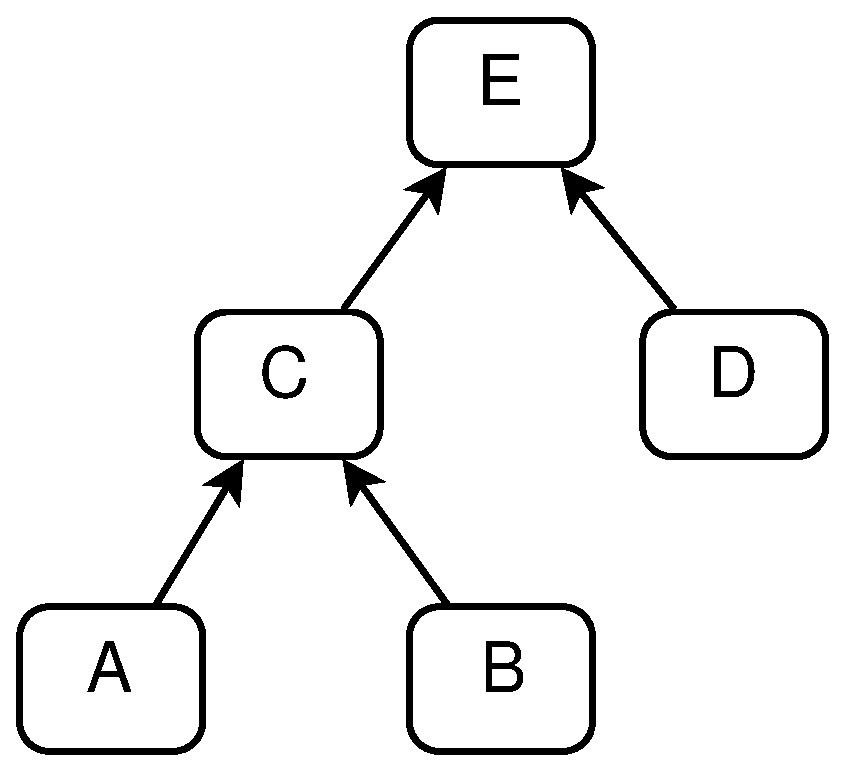
\includegraphics[width=.5\linewidth]{fig/simple-onto.eps}
\end{minipage}
\begin{minipage}[c]{.25\textwidth}\centering
    \begin{tabular}{ c | c | c | c | c | c |}
    \cline{2-6}
    	~ & A & B & C & D & E\\
    \cline{2-6}
    $A:$& 0 & 0 & 1 & 0 & 0 \\
    \cline{2-6}
    $B:$& 0 & 0 & 1 & 0 & 0 \\
    \cline{2-6}
    $C:$& 0 & 0 & 0 & 0 & 1 \\
    \cline{2-6}
    $D:$& 0 & 0 & 0 & 0 & 1 \\
    \cline{2-6}
    $E:$& 0 & 0 & 0 & 0 & 0 \\
    \cline{2-6}
    \end{tabular}
\end{minipage}
\begin{minipage}[c]{.25\textwidth}\centering
    \begin{tabular}{ c | c | c | c | c | c |}
    \cline{2-6}
    	~ & A & B & C & D & E\\
    \cline{2-6}
    $r_1:$& 1 & 1 & 0 & 0 & 0 \\
    \cline{2-6}
    $r_2:$& 1 & 1 & 1 & 0 & 0 \\
    \cline{2-6}
    $r_3:$& 0 & 1 & 1 & 0 & 0 \\
    \cline{2-6}
    $r_3:$& 0 & 0 & 0 & 1 & 0 \\
    \cline{2-6}
    \end{tabular}
\end{minipage}
\begin{minipage}[c]{0.4\linewidth}\centering
(A)
\end{minipage}
\begin{minipage}[c]{0.25\linewidth}\centering
(B)
\end{minipage}
\begin{minipage}[c]{0.25\linewidth}\centering
(C)
\end{minipage}
\caption{\label{fig:onto-and-data} Five concepts (\emph{A--E}) are represented visually as a hierarchy (A) and also as a a hypergraph using the binary feature matrix (B), where a ``1'' denotes \emph{rdfs:subClassOf}, which is similar to the ontology-annotated data (C), where ``1'' denotes \emph{mentions}.}
\end{figure*}

\begin{figure*}[tbh]
\begin{center}
\begin{tabular}{c  c}
\multirow{12}{*}{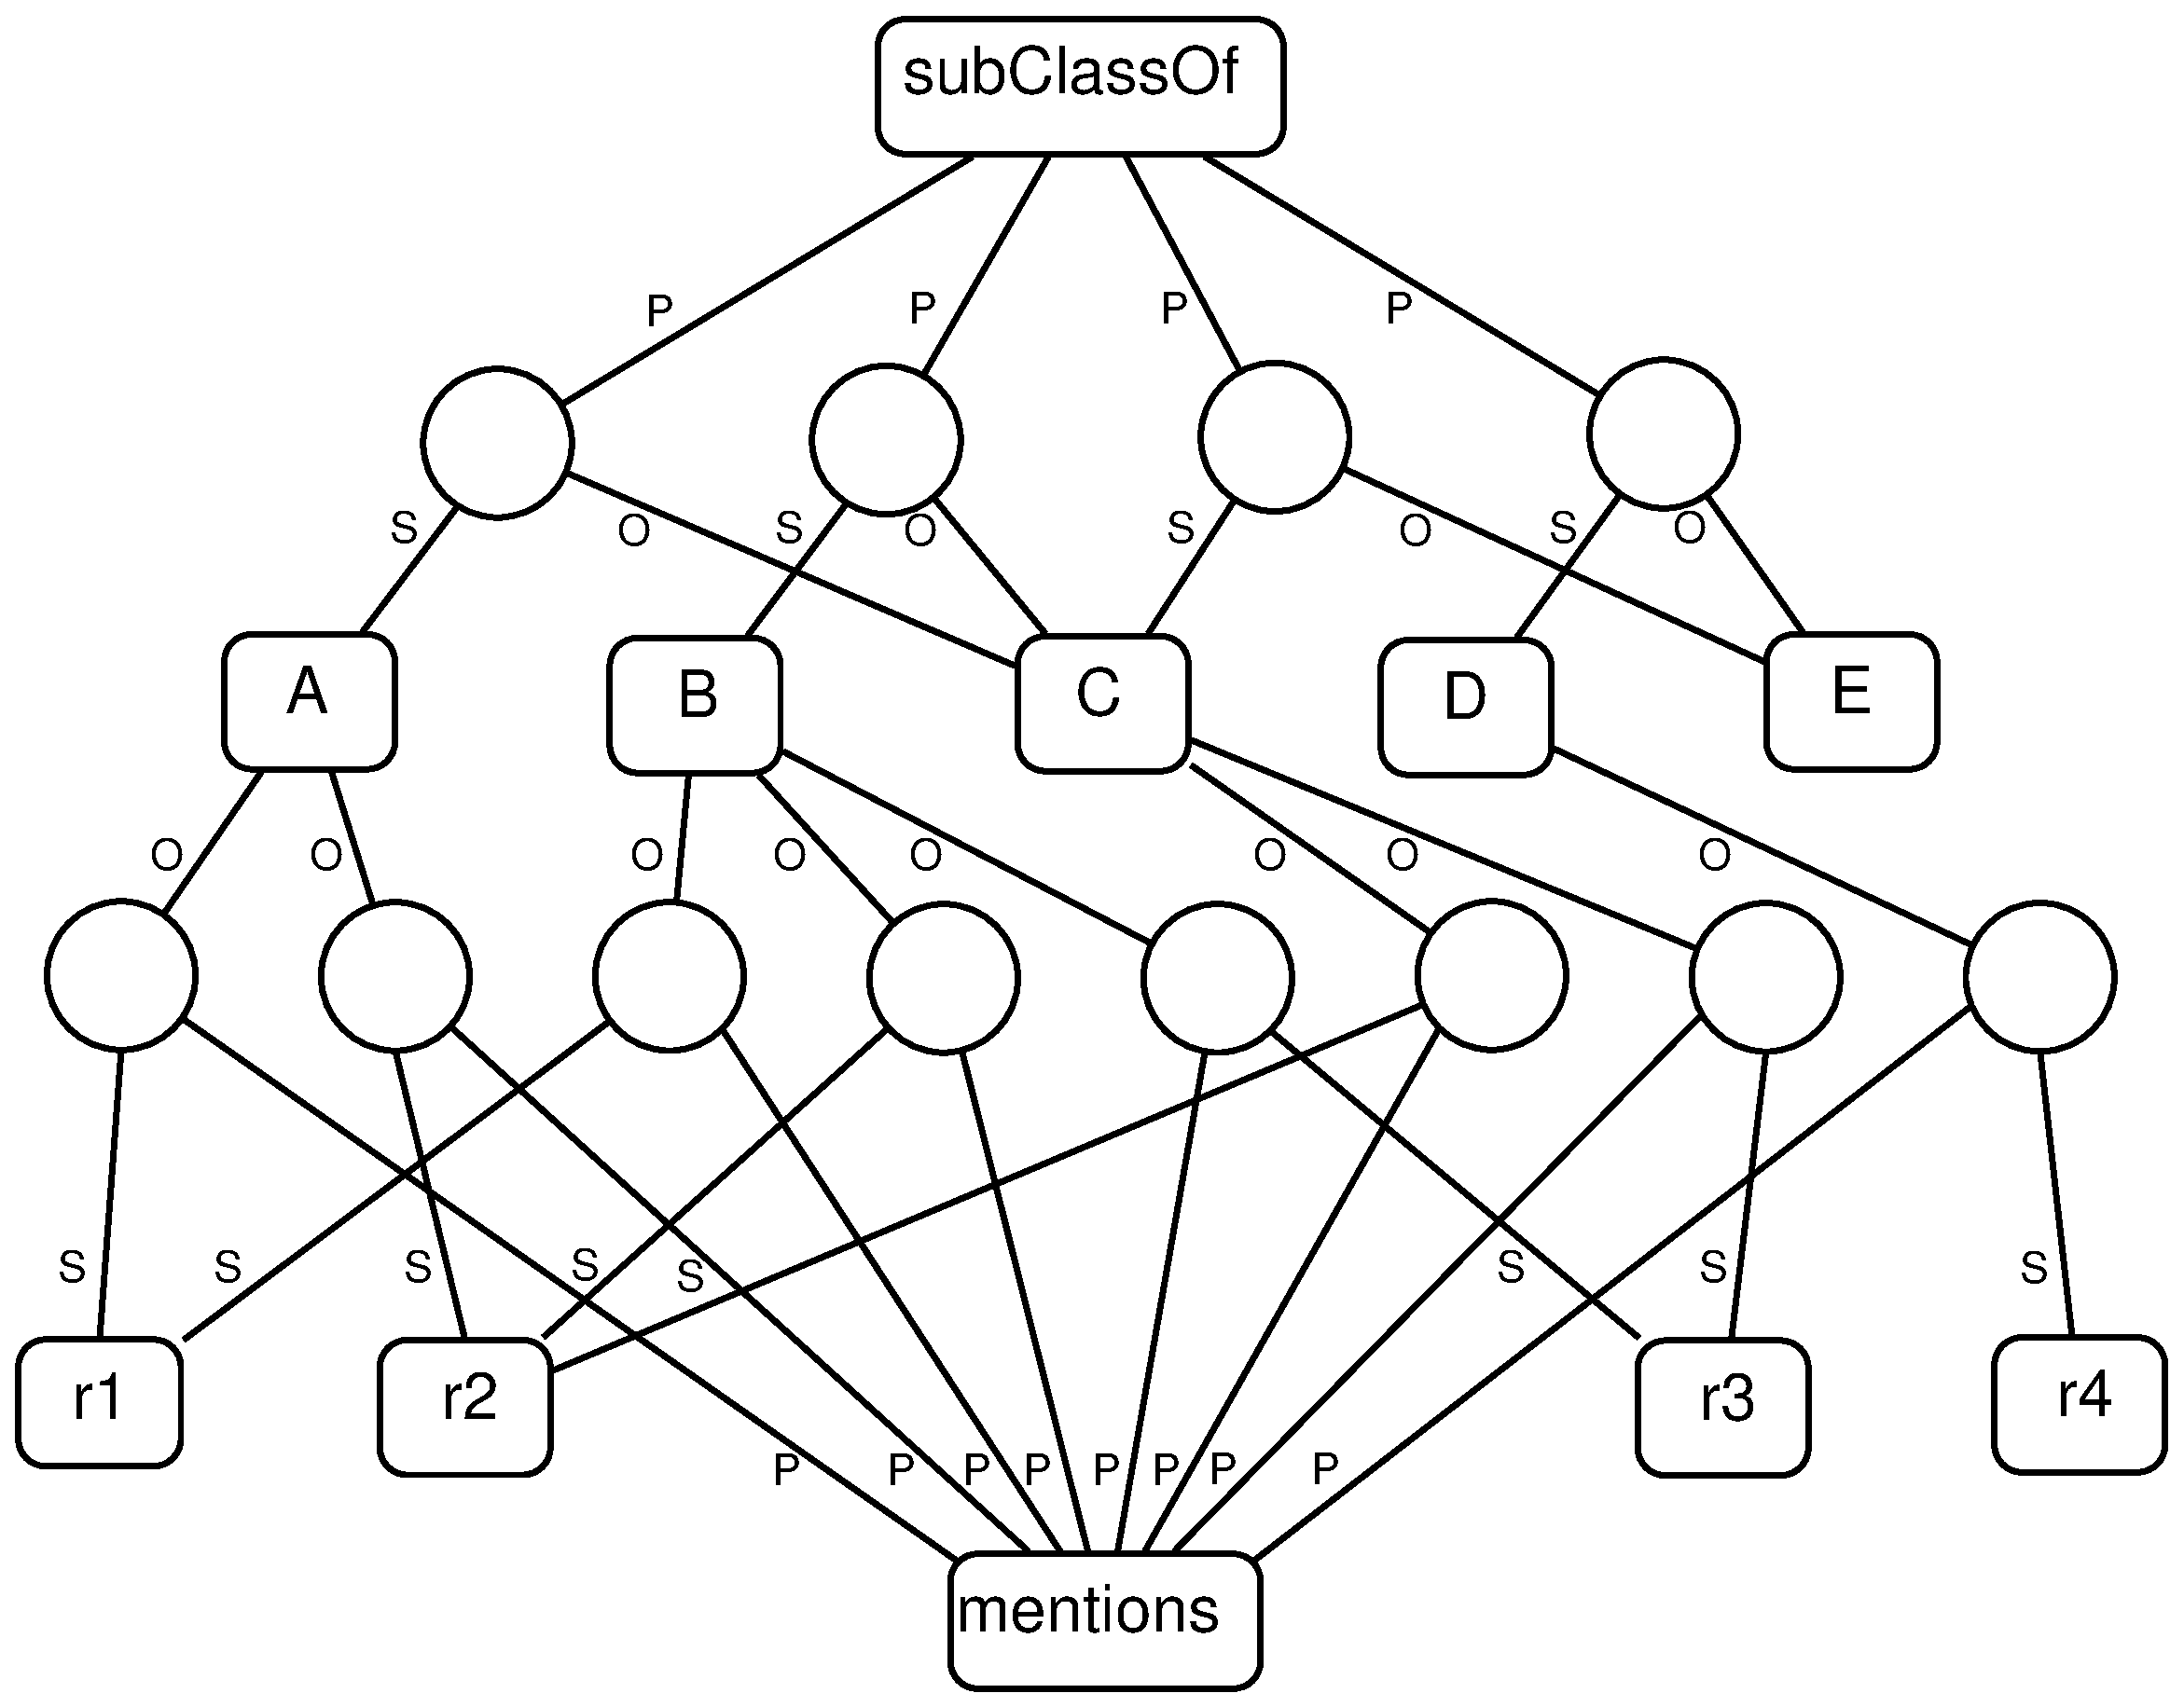
\includegraphics[width=.45\textwidth]{fig/hypergraph_mining.eps}} & \emph{~~~~~~~s \hfill p\hfill o~~~}\\
& $s_1$:~~~\texttt{<A>~~<subClassOf>~~<C>}\\
& $s_2$:~~~\texttt{<B>~~<subClassOf>~~<C>}\\
& $s_3$:~~~\texttt{<C>~~<subClassOf>~~<E>}\\
& $s_4$:~~~\texttt{<D>~~<subClassOf>~~<E>}\\
& \\
& $s_5$:~~~\texttt{<r1>\;~~<mentions>\;~~<A>}\\
& $s_6$:~~~\texttt{<r1>\;~~<mentions>\;~~<B>}\\
& $s_7$:~~~\texttt{<r2>\;~~<mentions>\;~~<A>}\\
& $s_8$:~~~\texttt{<r2>\;~~<mentions>\;~~<B>}\\
& $s_9$:~~~\texttt{<r2>\;~~<mentions>\;~~<C>}\\
& $s_{10}$:~~\texttt{<r3>\;~~<mentions>\;~~<B>}\\
& $s_{11}$:~~\texttt{<r3>\;~~<mentions>\;~~<C>}\\
& $s_{12}$:~~\texttt{<r4>\;~~<mentions>\;~~<D>}\\
& \\
& \\
& \\
& \\
(A) & (B)\\
\end{tabular}
\end{center}
\caption{\label{fig:hypergraph-combined} The RDF bipartite graph representation (A) easily combines both the ontology-annotated data with the ontological relationships (B) based on the information described in Figure~\ref{fig:onto-and-data}.}
\end{figure*}

In order to leverage the increasingly larger and richer collection of domain ontologies, especially in scientific fields such as the biomedical domain, we propose to use weights to distinguish paths in the RDF bipartite graph representing different semantic types or relationships (properties) from the ontology, such as class subsumption, ``part\_of", and other general or domain--specific properties. The weights also characterize the relative importance of the paths.

Formally, the RDF bipartite graph as a combined representation for both data and ontologies is defined as $G=\langle V_v \cup V_s, E \rangle$, where $V_v$ denotes \emph{value nodes} corresponding to components of RDF statements (i.e., subject, predicate, or object), and $V_s$ denotes \emph{statement nodes} corresponding to RDF statements. More specifically, statement nodes can be further divided according to whether they are from data or ontology, i.e., $V_s=V_d \cup V_o$; Value nodes can be divided according to whether they represent rows (records) or columns (attributes) in data, \i.e., $V_d=V_r \cup V_a$. The graph $G$ can be represented in a biadjacency matrix $\mathbf{M}$, where $\mathbf{M}(i,j)$ is non-zero if there is an edge between $\langle V_{v_i}, V_{s_j} \rangle$. For an unweighted graph, the value can be 0/1, and for a weighted graph, any non-negative value.
 
Figure~\ref{fig:biadjacency-matrices} shows the biadjacency matrices $\mathbf{M}_d$ and $\mathbf{M}_o$ for the data and ontology part of the RDF bipartite graph respectively. We can see that rows of $\mathbf{M}_d$ and $\mathbf{M}_o$ correspond to \emph{value nodes}, ($V_v$), which can be further divided into row nodes $V_r$ and attribute nodes $V_a$. On the other hand, columns of $\mathbf{M}_d$ are nodes that correspond to RDF statements about data ($V_d$), and columns of $\mathbf{M}_o$ correspond to the ontology ($V_o$). The union of $V_d$ and $V_o$ constitutes the whole set of statement nodes $V_s$ (circle nodes in Figure~\ref{fig:hypergraph-combined}(A).

\begin{figure*}[h!t]
\begin{center}
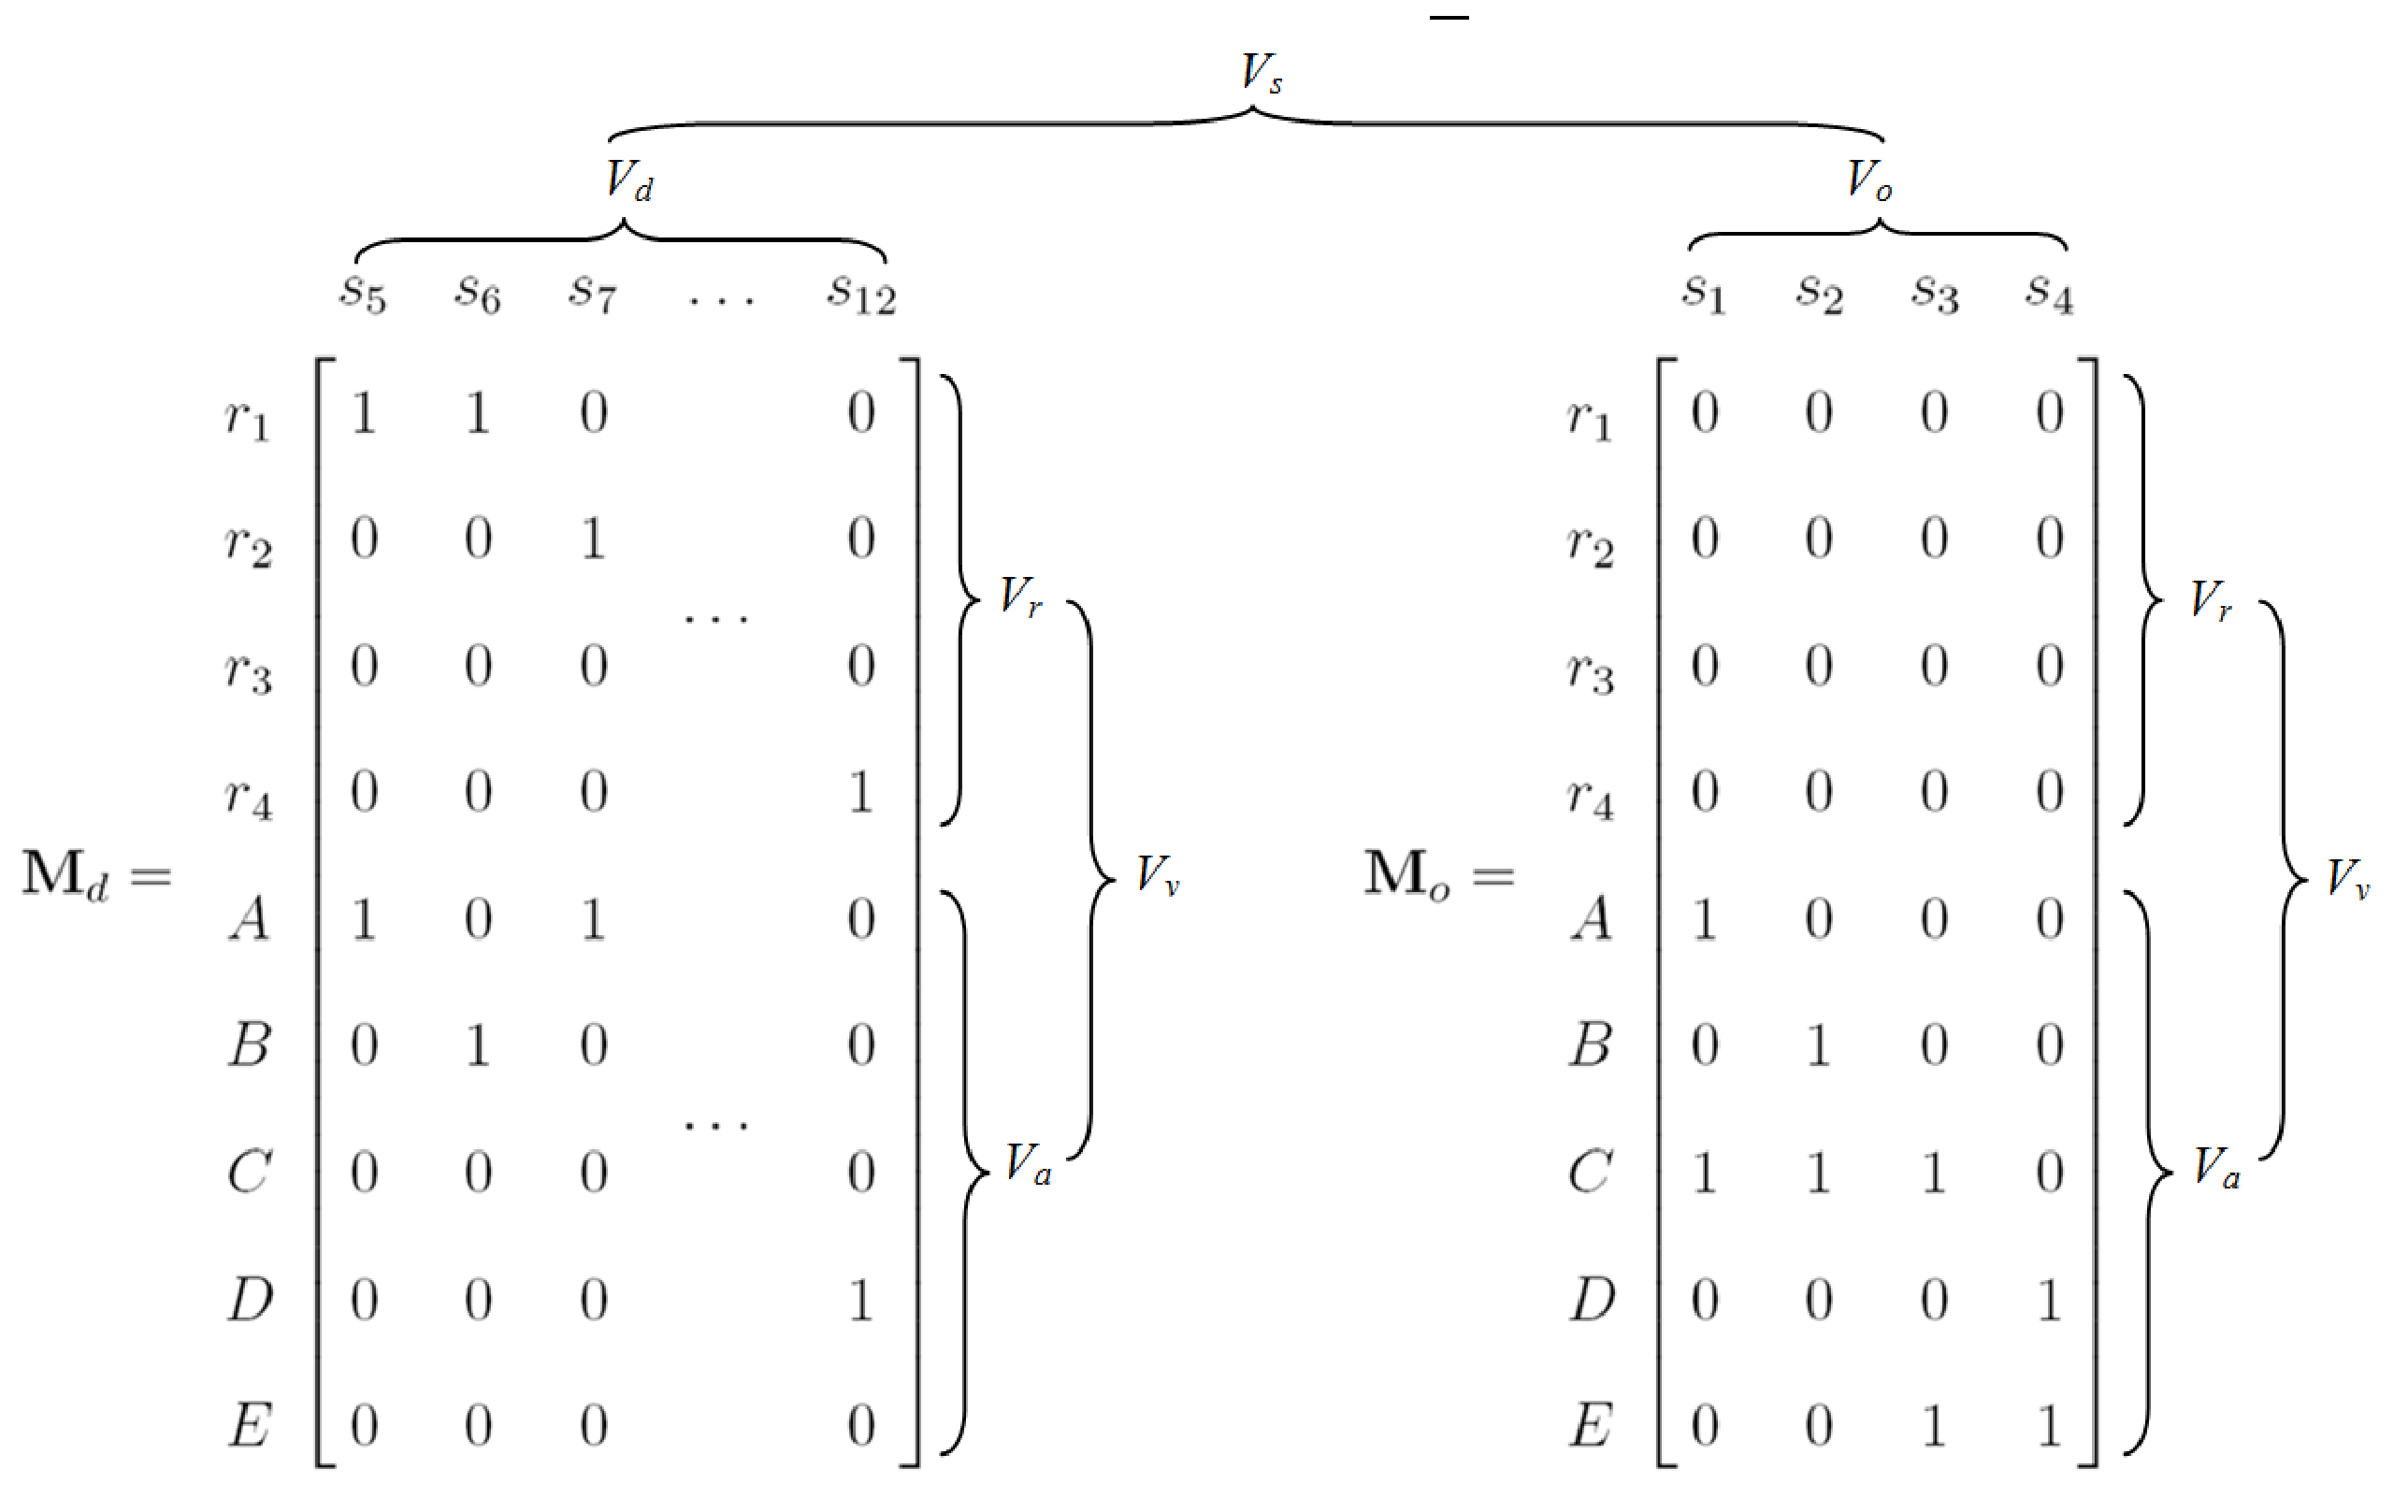
\includegraphics[width=.7\textwidth]{fig/biadjacency-matrices.eps}
\end{center}
\caption[An example RDF bipartite graph and a detailed anatomy of\protect\newline its biadjacency matrix]{\label{fig:biadjacency-matrices} An example RDF bipartite graph and a detailed anatomy of its biadjacency matrix.}
\end{figure*}


From the above example we notice that the biadjacency matrix $\mathbf{M}$ can be split into vertical stripes by statement nodes $V_s$. To obtain the biadjacency matrix $\mathbf{M}$ of the combined RDF bipartite graph in Figure~\ref{fig:biadjacency-matrices}(A), we can simply concatenate $\mathbf{M}_d$ and $\mathbf{M}_o$ horizontally: $\mathbf{M}=\left[\mathbf{M}_d~\mathbf{M}_o\right]$. This gives us a way to construct the matrix modularly from its independent components. In general, if there are $k$ different semantic relationships in ontologies, $\mathbf{M}_o$ can be divided into more vertical stripes $\{\mathbf{M}_{o_i}, i=1\dots k\}$, where $\mathbf{M}_{o_i}$ may represent, for example, the ``part\_of" lattice. Each $\mathbf{M}_{o_i}$ can be distinguished from others by different weights assigned to it. In short, $\mathbf{M}$ is the horizontal concatenation of all weighted vertical stripes as shown in~\ref{eq:horzcat}. The internal block structure of the concatenated biadjacency matrix $\mathbf{M}$ is shown in~\ref{striped_M}.

%horizontal concatenation
\begin{equation}\label{eq:horzcat}
\mathbf{M} = \bigg[w_d\mathbf{M}_d ~~ w_{o_1}\mathbf{M}_{o_1} ~~ w_{o_2}\mathbf{M}_{o_2} ~~ \dots\bigg]
\end{equation}

\begin{equation}
\label{striped_M}
\mathbf{M}=\begin{blockarray}{ccccc}
                ~ & ds & os_1 & os_2 & \dots \\
            \begin{block}{c[c|c|c|c]}
                r   &   \mathbf{M}_{dr}  &   \mathbf{0}   &   \mathbf{0}   &   \dots \\
                \cline{2-5}
                a   &   \mathbf{M}_{da}  &   \mathbf{O}_1 &   \mathbf{O}_2 &   \dots \\
            \end{block}
        \end{blockarray}
\end{equation}


%By developing the unified representation for both data and domain knowledge, and utilizing ontology annotations (\eg,~\cite{LePendu2010}), we can produce a unified RDF bipartite graph, which serves as the basis for mining semantically associated itemsets. With additional information from domain knowledge encoded in ontologies, the unified RDF bipartite graph enables us to discover interesting indirect relationships between entities from data. Moreover, the same method also makes it possible to validate relationships between ontological concepts with the help of the present data graph. In the next section, we describe a similarity measure based on random walk with restart on the RDF bipartite graph to capture the semantic association.

With the RDF bipartite graph and the form of its biadjacency matrix defined, in the following, we move on to describe a similarity measure based on random walk with restart over this graph to discover semantically associated itemsets.


\subsection{Similarity Ranking by Random Walk with Restart}

Similar to the relevance score~\cite{SunEtal05}, we believe that two items have a strong semantic association if they are related to many similar objects. We denote the similarity score between entities $e_1$ and $e_2$ by $s(e_1, e_2)$, where $s(e_1,e_2) \in [0, 1]$ and $s(e_1, e_2) = 1 \text{ if } e_1 = e_2$. Now the problem of ranking semantic associations in the unified graph can be described as follows.

Given an attribute node $a$ in the unified graph $G = G_d \cup G_o$ and $a \in G_d \cap G_o$ we want to compute a similarity score $s(a, b)$ for all nodes $b(\neq a) \in G_d \cap G_o$. The result is a one-column vector containing all similarity scores with respect to $a$~\cite{Chen_tuplerank:ranking}. We choose to apply random walks with restart (RWR) from the given node $a$, and use the steady-state probability of each other node at convergence as the similarity measure. In other words, the similarity score of node $b$ is defined as the probability of visiting $b$ via a random walk which starts from $a$ and goes back to $a$ with a probability $c$.

%RWR is closely related to the two similarity measures, i.e., $s_{CT}$ and $s_{L+}$, that are presented in Chapter~\ref{chap:datamining} on RDF hypergraphs, since they are all derived from the random walk model. It is sometimes a desirable property of a similarity measure for many applications, if it is able to discount nodes with large degrees like the $s_{L+}$ measure. The adaptation of $s_{L+}$ to RDF bipartite graph is a topic worth exploring in future work. However, the scores of RWR on bipartite graphs are easier to compute, especially, when the number of nodes in the two sides is highly unbalanced. The RDF bipartite graph is unbalanced because there are generally many more statement nodes than value nodes on large graphs. Therefore we focus on studying RWR over the RDF bipartite graph in this chapter.

In more detail, RWR in a bipartite graph works as follows: assume we have a random walker that starts from node $a$. For each step, the walker chooses randomly among the available edges from the current node. After each iteration, with probability $c$, it resets its position back to node $a$. The final steady-state probability that the random walker reaches node $b$ is the similarity score of $b$ with respect to $a$. We choose the random walk approach to compute the relevance score because it gives node $b$ high ranking if $b$ and $a$ are connected by many nodes; this is due to the random walker having more paths to reach $b$ from $a$. The purpose of the periodic restart of the random walk is to raise the chance that close related nodes are visited more often than other nodes.

In the following, we describe how to calculate algorithmically the similarity ranking based on random walk with restart on the unified RDF bipartite graph. The algorithm can be used in situations where, for example, users are interested in knowing products that are usually bought together in the same transactions by different customers, or common side effects of the same drugs prescribed to different patients, etc.

Given a biadjacency matrix $\mathbf{M}$ in~\ref{eq:horzcat} for the combined RDF bipartite graph $G$, we can construct the adjacency matrix $\mathbf{A}$ of $G$ as following:
\[
\mathbf{A}=\left[
               \begin{array}{cc}
                 \mathbf{0}   & \mathbf{M} \\
                 \mathbf{M}^T & \mathbf{0} \\
               \end{array}
             \right].
\]
The probability of a random walker taking a particular edge $\langle a,b\rangle$ from a node $a$ while traversing the graph is proportional to the edge weight over the total weight of all outgoing edges from $a$, i.e., $\mathbf{P}(a,b)=\mathbf{A}(a,b)/\Sigma_{i=1}^{m+n}\mathbf{A}(a,i)$. Therefore, the Markov transition matrix $\mathbf{P}$ of $G$ is constructed as: $\mathbf{P}=normc(\mathbf{A})$, where $normc(\mathbf{A})$ normalizes $\mathbf{A}$ such that every column sum up to 1.

Given the transition matrix $\mathbf{P}$, we can calculate the similarity scores using the following steps. First, we transform the input attribute node $a$ into a $(k+n) \times 1$ query vector $\mathbf{q}_a$ with 1 in the $a$-th row and 0 otherwise. Second, we need to compute a $(k+n)\times 1$ steady-state probability vector $\mathbf{u}_a$ over all nodes in $G$. Last we extract only the steady-state probabilities of row nodes in $\mathbf{M}$ (corresponding to value nodes in the RDF bipartite graph) as the output similarity score vector. Notice that $\mathbf{u}_a$ can be computed by an iterated method from the following iterative equation.

Let $c$ be the probability of restarting random-walk from the node $a$. Then the steady-state probability vector $\mathbf{u}_a$ satisfies
\begin{equation}
\label{eq:steady-state}
\mathbf{u}_a=(1-c)\mathbf{P}_A\mathbf{u}_a+c\mathbf{q}_a~.
\end{equation}

\renewcommand{\algorithmicrequire}{\textbf{Input:}}
\renewcommand{\algorithmicensure}{\textbf{Output:}}
\begin{algorithm}
\caption{Calculate Semantic Association}
\label{alg1}
\begin{algorithmic}
\REQUIRE query attribute $a$, bipartite matrix $M$, restarting probability $c$, tolerant threshold $\epsilon$
\ENSURE similarity vector $\mathbf{u}_a(1:k)$
\STATE $\mathbf{q}_a \Leftarrow \mathbf{0}$
\STATE $\mathbf{q}_a(a)=1$ (set $a$-th element of $\mathbf{q}_a$ to 1)
\WHILE{$|\Delta\mathbf{u}_a| > \epsilon$}
\STATE \[
    \mathbf{u}_a = (1-c)  \left[ \begin{array}{c}
        normc(\mathbf{M})\mathbf{u}_a(k+1:k+n);\\
        normc(\mathbf{M}^T)\mathbf{u}_a(1:k)
    \end{array} \right] + c\mathbf{q}_a
\]
\ENDWHILE
\RETURN $\mathbf{u}_a(1:k)$
\end{algorithmic}
\end{algorithm}

The iterative update of $\mathbf{u}_a$ can be performed as shown in Algorithm~\ref{alg1}. The while loop is modified from~\ref{eq:steady-state} to avoid materializing $\mathbf{A}$ and $\mathbf{P}$ for scalability. 
\section{Experiment}
\label{experiment}
In this section, we evaluate the method of random walk with restart on the unified RDF bipartite graph for discovering semantic associations and detecting misinformation in biomedical ontologies. We conducted a series of experiments to demonstrate the effect of the incorporating the ontologies in the mining task. We evaluated our methods on an \emph{electronic health records} dataset to highlight its scalability and applicability for problems in the biomedical domain.

\subsection{Dataset}
In this evaluation, we analyze the electronic health records of real patients. The clinical note data are from Stanford Hospital's Clinical Data Warehouse (STRIDE). These records archive over 17-years worth of data comprising of 1.6 million patients, 15 million encounters, 25 million coded ICD9 diagnoses, and a combination of pathology, radiology, and transcription reports totaling over 9 million clinical notes (i.e., unstructured text).
We obtained the set of drugs and diseases for each patient's clinical note by using a new tool, the \emph{Annotator Workflow}, developed at the National Center for Biomedical Ontology (NCBO), which annotates clinical text from electronic health record systems and extracts disease and drug mentions from the electronic health records.


One strength of the Annotator is the highly comprehensive and interlinked lexicon that it uses. It can incorporate the entire NCBO BioPortal ontology library of over 250 ontologies to identify biomedical concepts from text using a dictionary of terms generated from those ontologies. Terms from these ontologies are linked together via mappings. For this study, we specifically configured the workflow to use a subset of those ontologies that are most relevant to clinical domains, including Unified Medical Language System (UMLS) terminologies such as SNOMED-CT, the National Drug File (NDFRT) and RxNORM, as well as ontologies like the Human Disease Ontology. The resulting set of ontologies contains 1 million subsumption statements.

From this set of 1.6 million patients with annotated records, we vectorize texts and turned them into a huge bag-of-word representation, from which an RDF bipartite graph is constructed, including 148 million RDF statements for the data.

To highlight the capability of our method for incorporating multiple types of relationships, we also explore the ``may\_treat" relationship between drugs and diseases defined in the NDFRT ontology, for example, Thiabendazole ``may\_treat" Larva Migrans. In the experiment, we extracted 43,780 may\_treat statements from the ontology. Since we are interested in learning the interaction between drugs and diseases, may\_treat is naturally a better indicator relationship to include while mining semantic associations than the subsumption relationship. Our results below illustrate this point.

We applied our algorithms to all previous records in the patient's timeline, looking at just the set of drugs and their semantically related diseases. Therefore, at a very simplistic level, the experiment result shows that strong semantic associatoins in this context could possibly represent sets of drugs that could lead toward certain diseases. To summarize, the size of the dataset in terms of numbers of RDF statements in the bipartite graph is shown in Table~\ref{tbl:exp_overview}.


\begin{table}[tbh]\scriptsize
\begin{center}
\begin{tabular}{c|c|c}
\hline
  \# data stmts & \# is\_a stmts & \# may\_treat stmts \\
  \hline
  148,690,056  & 1,048,604 &    43,780\\
  \hline
\end{tabular}
\end{center}
\caption{\label{tbl:exp_overview} Numbers of RDF statements in the unified bipartite graph extracted from the electronic health dataset. }
\end{table}


\subsection{Results}
\subsubsection{Discovering Semantic Associations}
Before studying the drug-disease association, we first carried out a study on the drug-drug association. To this purpose, we combine the subsumption hierarchy in the ontology graph with the data graph. Table~\ref{tbl:health_comp} demonstrates semantic association with the term \emph{rofecoxib} given different configurations of the unified graphs. Rofecoxib is the active ingredient of the drug \emph{Vioxx}, which was recalled in 2005 because it was causing an increased risk of heart attacks. Vioxx is one of several non-steroidal anti-inflammatory drugs part of the COX-2 inhibitor class of drugs.

Table~\ref{tbl:health_comp} shows that, with only the ontology graph, the algorithm successfully picks up almost all other active ingredients part of the COX-2 inhibitor class of drugs (valdecoxib, celecoxib, etc.). Drugs of the COX inhibitor (the parent of COX-2) class also appear in the top results (meloxicam, nabumetone, etc.). These are indeed semantic associations since the top items are related to rofecoxib indirectly through parent classes. It is worth noticing that, although rofecoxib is a subclass of COX-2 inhibitor drugs, it is also a derived class from a much broader parent called ``Drug Products by Generic Ingredient Combinations," whose subclasses are organized by descendants' initial alphabets. In other words, rofecoxib is a direct child of a class that contains all drug ingredients starting with the letter R. The fact that our algorithm selects the neighboring class of rofecoxib in the COX-2/COX family instead in the R-initialed family demonstrates its capability of discovering interesting and meaningful semantic associations. An ontology inference engine that is able to derive sibling classes would never be able to achieve the same meaningful ranking as our algorithm does in this case.

Without any preprocessing and prior knowledge about how the clinical notes are prescribed, the results with data graph alone do not seem to have a strong pattern because of the appearance of too many general terms. However, the noteworthy inclusion of ``reflux" and ``infantile" may be due to the causal relationships between rofecoxib and acid reflux and infantile gastroenteritis respectively that have been shown in previous studies. Applying general information extraction techniques, such as pruning out general terms (``medical history, " ``today," etc.) should be able to improve the performance with data graph alone.

On the other hand, adding the is\_a graph to the data graph can be also seen as a mean for denoising and enhancement of the data. In the results with both data and is\_a graphs, valdecoxib and celecoxib are promoted to the top results. This suggests that the evidences from both data and ontology conforms with previous studies in which celecoxib, valdecoxib are shown to be, similar to rofecoxib, also associated with increased risk of cardiovascular pathologies.

\begin{table*}[htbp]\scriptsize
\begin{center}
\begin{tabular}{ c | c | c | c  }
\hline
rank    &   w/ data only	&	w/ is\_a only		& w/ both data and is\_a \\
\hline
1	&		reflux	&	valdecoxib	&		reflux	\\
2	&		medical history	&	meloxicam	&		obstruction	\\
3	&		history of previous events	&	celecoxib	&		injury	\\
4	&		diagnosis	&	parecoxib	&		valdecoxib	\\
5	&		pharmaceutical preparations	&	etoricoxib	&		medical history	\\
6	&		blood and lymphatic system disorders	&	deracoxib	&		foreign body sensation	\\
7	&		disease	&	lumiracoxib	&		history of previous events	\\
8	&		infantile neuroaxonal dystrophy	&	firocoxib	&		adverse effects	\\
9	&		today	&	nabumetone	&		celecoxib	\\
10	&		hypersensitivity	&	macrolides	&		actual hypothermia	\\
\hline
\end{tabular}
\end{center}
\caption[Top results on the electronic health dataset]{\label{tbl:health_comp}Results of items ranked by the strength of semantic association with the term ``rofecoxib."}
\end{table*}

To verify the drug-disease association and study the impact of different semantic relationships on finding such association, we carry out the following experiment. Table~\ref{tbl:health_exp} illustrates the rankings of three associations (one per row) under different settings (data alone, data plus is\_a, and data plus may\_treat, respectively). The first element in the pair is the query item, which are all active ingredients of some prescription drugs, and the ranking shown in the table is for the second item, which are diseases. For example, arthritis is ranked as the 527th semantic association to rofecoxib according to similarity ranking based only on data graph. All these item pairs are actually gold standard associations backed by known drug-disease relationships, we know the strength of associations between them should be strong.

We observe that the ranking based on data graph alone is fairly high already, consider there are approximately 1 million concepts of interest. However, the results based on the combination of data and subsumption (``is\_a") graph are worse. It is because the subsumption hierarchies for drugs and diseases are largely separate structures. Therefore the subsumption relationships can only boost the association within the drug and disease hierarchies respectively, but obfuscate the cross-hierarchy associations that we aim to find between drugs and diseases. On the other hand, however, the association between these pairs can be exactly captured by the NDFRT ``may\_treat" relationship (e.g., NDFRT explicitly defines that rofecoxib ``may\_treat" arthritis). When the ``may\_treat" graph is incorporated into the mining process, the ranking for the association is greatly boosted.


\begin{figure}[htbp]
\begin{minipage}[c]{0.49\textwidth}\centering
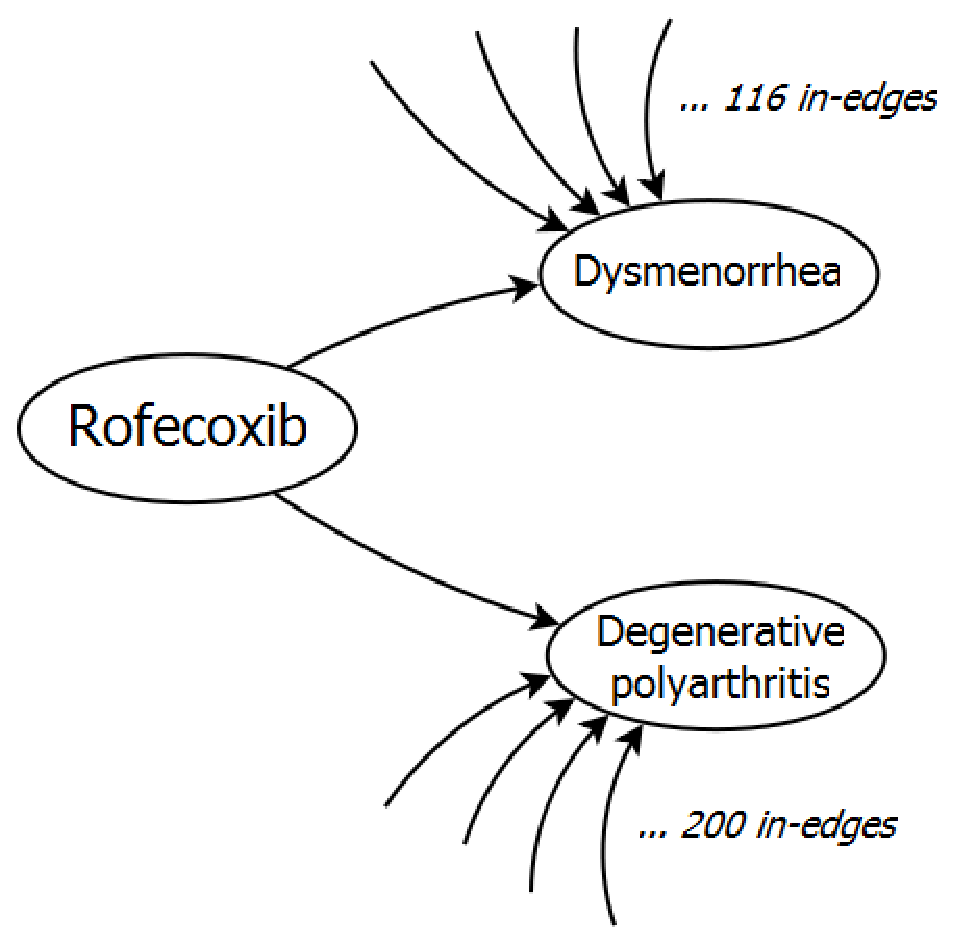
\includegraphics[width=.54\textwidth]{fig/may_treat.eps}
\end{minipage}
\begin{minipage}[c]{0.49\textwidth}\centering
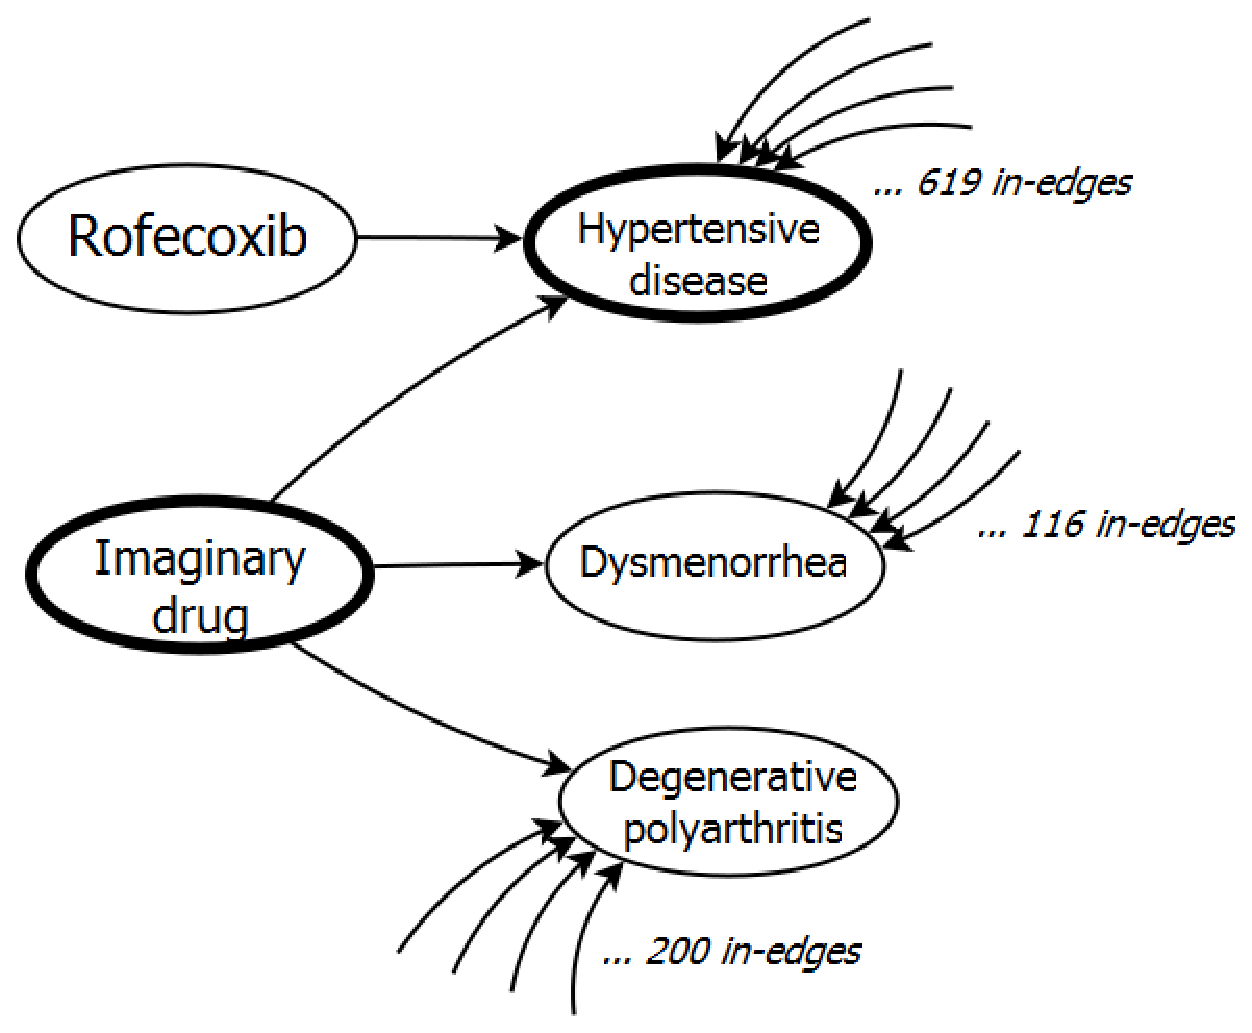
\includegraphics[width=.7\textwidth]{fig/may_treat_augmented.eps}
\end{minipage}
\caption[The may\_treat subgraph]{\label{fig:may_treat} The upper part of the figure shows the ground-truth may\_treat relationships between the drug rofecoxib and two diseases. The lower part shows the same subgraph with deliberate falsehoods.}
\end{figure}

\subsubsection{Detecting Misinformation in Ontologies}
Conversely, we are also interested in learning whether the data graph can help discover misinformation in ontologies. Figure~\ref{fig:may_treat} (upper) shows a subgraph of the NDFRT ``may\_treat" relationship. According to the ontology, rofecoxib can treat two diseases, namely, dysmenorrhea and degenerative polyarthritis. There are also 116 and 200 other drugs known to treat dysmenorrhea and degenerative polyarthritis respectively (hence the in-degrees of the nodes). To simulate an imperfect ontology, we alter the ground truth graph by introducing some deliberate misinformation and falsehoods, as shown in Figure~\ref{fig:may_treat} (lower). In more details, we specify that rofecoxib may treat hypertensive disease, which in fact can be treated by the most number of drugs (619 in total) according to the NDFRT ontology. Then we add another imaginary drug to treat degenerative polyarthritis, dysmenorrhea, and hypertensive disease. In this way, the original immediate connections between rofecoxb and degenerative polyarthritis and dysmenorrhea become erroneously indirect and are obfuscated by the noise of high-degree nodes along the path. With this setup, we hope to learn if the incorporation of data graph can help correct the ontology.


\begin{table*}[htbp]\scriptsize
\begin{center}
\begin{tabular}{ c | c  c | c  c | c  c }
\hline
\multirow{2}{*}{~}        &   \multicolumn{2}{c|}{w/ data only}  &   \multicolumn{2}{c|}{w/ data and ``is\_a"} & \multicolumn{2}{c}{w/ data and ``may\_treat"}\\
\cline{2-7}
                        	&   p(\%)   &   rank    &   p(\%)    &   rank    &   p(\%)    &    rank    \\
\hline
$\langle rofecoxib, degenerative~polyarthritis\rangle$  &   0.006   &   527     &   0.004    &   632     &   0.51     &     13     \\
$\langle valdecoxib, degenerative~polyarthritis\rangle$  &   0.007   &   613     &   0.005    &   695     &   0.63     &     17     \\
$\langle troglitazone, diabetes\rangle$  &   0.006   &   478     &   0.005    &   514     &   0.44     &     11     \\
\hline
\end{tabular}
\end{center}
\caption[Rankings of three semantic associations in health data under different settings]{\label{tbl:health_exp}Rankings of three semantic associations under different settings.}
\end{table*}

\begin{table*}[htbp]\scriptsize
\begin{center}
\begin{tabular}{ c | c  c | c  c }
\hline
\multirow{2}{*}{~}  &   \multicolumn{2}{c|}{w/ noisy may\_treat only}    &   \multicolumn{2}{c}{w/ data and noisy may\_treat}\\
\cline{2-5}
       	&   p(\%)   &   rank    &  p(\%)    &    rank    \\
\hline
$\langle rofecoxib, degenerative~polyarthritis\rangle$       &   3.60e-3   &   555     &   8.14e-3    &   263    \\
$\langle rofecoxib, dysmenorrhea\rangle$    &   1.54e-2   &   246     &   1.26e-3    &   1703   \\
\hline
\end{tabular}
\end{center}
\caption[Rankings of associations on the noisy may\_treat graph]{\label{tbl:salted_may_treat}Rankings of associations on the noisy may\_treat graph (Figure~\ref{fig:may_treat} right) between Rofecoxib and two diseases derived with and without data.}
\end{table*}

Table~\ref{tbl:salted_may_treat} shows the result of ranks of the associations between rofecoxib and degenerative polyarthritis and dysmenorrhea respectively. The ranks of the associations drastically drop to the 555th and 246th respectively on the noisy graph from the top two on the original ground truth graph. This is mainly due to the presence of a large node, hypertensive disease, in the middle of the connections. However, with the unified data and may\_treat graph, we notice that the rank of rofecoxib and degenerative polyarthritis increases to 263rd, while the rank of rofecoxib and  dysmenorrhea decreases to 1703rd. This shows that the data graph endorses more strongly the association between rofecoxib and degenerative polyarthritis. Indeed, although rofecoxib are known to treat both degenerative polyarthritis and dysmenorrhea, the former is a much more popular usage. A search on the National Library of Medicine's PubMed database\footnotemark[1] for ``rofecoxib and polyarthritis" returns 518 results, while ``rofecoxib and dysmenorrhea" only returns 29. This result shows that the data graph can help correct misinformation in ontologies to some extent, and in a sense, it also gives a clue of how prior beliefs fit with reality.

\footnotetext[1]{\url{http://www.ncbi.nlm.nih.gov/}}


%\section{Discussion}
\label{sec:discussion}
We have demonstrated that using the proposed combined RDF bipartite graph incorporates both domain knowledge and data based on the user's desired weights for each component for finding \emph{semantically associated itemsets}.

Developing scalable algorithms for semantic data mining is critically important. In our work, the healthcare dataset has grown beyond 100 billion triples and the size of the ontologies used are also large (SNOMED-CT has nearly 400,000 classes). The RWR method we describe works well for query-based node similarity, but it will not scale to generate full pair-wise node similarities at this tremendous scale because a calculation of eigenvectors of the Laplacian is required to derive the similarity measures, which is very expensive on large graphs. While non-trivial practical problems associated with very large graphs cannot be completely avoided, our work makes it possible to leverage decades of work on graph-based methods in this effort to mine semantically associated data. A promising direction going forward is to employ approximation and develop parallelizable algorithms.

The weighted hyperedges provide a great deal of flexibility to users who may prefer domain knowledge over data (or vice versa) and opens up new research questions on how to optimally configure learning algorithms. In reality, the appropriate ratio for the edge weights is not only dependent on the size of graphs but also the graph configuration (depth, average degree, etc). Moreover, allowing users to specify the ratio of prior knowledge in ontologies versus inductive evidence from data enables us to discover empirically optimal configurations. We have performed exhaustive feature selection on classification algorithms for our healthcare dataset in the past, and we would also explore a few permutations on these hyperedge weights going forward.

The RDF bipartite graph representation has limited expressivity compared to OWL itself. For example, domain, range and cardinality constraints are not straightforward to model.  One possible approach is to model domain constraints by explicitly describing the desired or acceptable walk (traversal sequence) in the RDF hypergraph. In this case, the recently proposed \emph{regular traversal expression} ~\cite{Marko10} technique may apply. However, their fast power-iteration approach for computing the stationary probability may not be applicable any more due to the label sequence constraint, but the Monte-Carlo simulation of the random walk may help to approximate the similarity measure.
\section{Conclusion and Future Work}
\label{sec:conclusion}

%We approach the discovery of indirectly associated items from ontology-annotated data, called \emph{semantically associated itemsets}, by proposing a new semantic data mining technique.  Our method uses hypergraphs and random walks with restart over a bipartite graph serialization to discover associations that cannot be found by methods that rely on co-frequent items because it utilizes both the ontology and the data at the same time.  Moreover, we allow users the ability to customize the weight of each component, giving flexibility in how strongly the role of the ontology plays over the data, or vice-versa.  Our evaluations show that the method discovers indirect associations and that it scales to datasets that are large in multiple says: the ontology can be large and the data can be large.
%
%In future work, we will explore algorithms that suggest appropriate weights to apply to the components of the hypergraph. Also, we will implement methods for clustering and classification tasks within this framework. We will focus on our healthcare datasets mainly because they are both large and complex, but also because of the enormous potential in advancing the state-of-the-art in clinical informatics and improving the quality of care for millions of patients.

We mine biomedical ontologies and  data using a unified RDF hypergraph representation.  Our method uses random walks with restart over a bipartite graph serialization to discover semantic (indirect) associations that cannot be found by methods that rely on co-frequencies because our method utilizes both the ontology and the data at the same time. We are one of the first research groups which consider to mine biomedical ontologies and data together without using a separate system to pre-processing or pre-computing ontologies. We allow users the ability to customize the weight of each component, giving flexibility in how strongly the role of the ontology plays over the data, or vice-versa.  Our evaluations show that the method discovers semantic associations and that it scales to datasets that are large in multiple says: the ontology can be large and the data can be large. Moreover, we also show that our data mining methods can discover the errors in biomedical ontologies injected by human operations.

In the following we highlight some future research directions in mining the unified RDF bipartite graph.

Developing scalable algorithms for semantic data mining is critically important. The healthcare dataset in our study has grown beyond 100 billion triples and the size of the ontologies used are also large (SNOMED-CT has nearly 400,000 classes). The RWR method we describe works well for query-based node similarity, but it will not scale to generate full pair-wise node similarities at this tremendous scale because a calculation of eigenvectors of the Laplacian is required to derive the similarity measures, which is very expensive on large graphs. While non-trivial practical problems associated with very large graphs cannot be completely avoided, our work makes it possible to leverage decades of work on graph-based methods in this effort to mine semantically associated data. A promising direction going forward is to employ approximation and develop parallelizable algorithms.

The weighted hyperedges provide a great deal of flexibility to users who may prefer domain knowledge over data (or vice versa) and opens up new research questions on how to optimally configure learning algorithms. In reality, the appropriate ratio for the edge weights is not only dependent on the size of graphs but also the graph configuration (depth, average degree, etc). Moreover, allowing users to specify the ratio of prior knowledge in ontologies versus inductive evidence from data enables us to discover empirically optimal configurations. We have performed exhaustive feature selection on classification algorithms for our healthcare dataset in the past, and we would also explore a few permutations on these hyperedge weights going forward.

The RDF bipartite graph representation has limited expressivity compared to OWL itself. For example, domain, range and cardinality constraints are not straightforward to model.  One possible approach is to model domain constraints by explicitly describing the desired or acceptable walk (traversal sequence) in the RDF hypergraph. In this case, the recently proposed \emph{regular traversal expression} ~\cite{Marko10} technique may apply. However, their fast power-iteration approach for computing the stationary probability may not be applicable any more due to the label sequence constraint, but the Monte-Carlo simulation of the random walk may help to approximate the similarity measure.

We will continue to focus on healthcare datasets mainly because large number of biomedical ontologies have been developed and used to annotate the real-life data, but also because of the enormous potential in advancing the state-of-the-art in clinical informatics and improving the quality of care for millions of patients. This research also contributes to an emerging research direction of semantic data mining, in which formal semantics that exist in data and knowledge can be represented and incorporated into the data mining process in a seamless way.





%ACKNOWLEDGMENTS are optional
%\input{Acknowledgments}

\bibliographystyle{abbrv}
\bibliography{dou,prop,thesis,paea}



\end{document}
